%%%%%%%%%%%%%%%%%%%%%%%%%%%%%%%%%%%%%%%%% % a0poster Landscape Poster % LaTeX Template % Version 1.0 (22/06/13) % % The a0poster class was created by: % Gerlinde Kettl and Matthias Weiser (tex@kettl.de) % % This template has been downloaded from: % http://www.LaTeXTemplates.com % % License: % CC BY-NC-SA 3.0 (http://creativecommons.org/licenses/by-nc-sa/3.0/)
%
%%%%%%%%%%%%%%%%%%%%%%%%%%%%%%%%%%%%%%%%%

%----------------------------------------------------------------------------------------
%	PACKAGES AND OTHER DOCUMENT CONFIGURATIONS
%----------------------------------------------------------------------------------------

\documentclass[a0,landscape]{a0poster}

\usepackage{multicol} % This is so we can have multiple columns of text side-by-side
\columnsep=100pt % This is the amount of white space between the columns in the poster
\columnseprule=3pt % This is the thickness of the black line between the columns in the poster

\usepackage[svgnames]{xcolor} % Specify colors by their 'svgnames', for a full list of all colors available see here: http://www.latextemplates.com/svgnames-colors

%\usepackage{times} % Use the times font
\usepackage{palatino} % Uncomment to use the Palatino font
%\usepackage{ClearSans}

\usepackage{graphicx} % Required for including images
\graphicspath{{figures/}} % Location of the graphics files
\usepackage{booktabs} % Top and bottom rules for table
\usepackage[font=small,labelfont=bf]{caption} % Required for specifying captions to tables and figures
\usepackage{amsfonts, amsmath, amsthm, amssymb} % For math fonts, symbols and environments
\usepackage{wrapfig} % Allows wrapping text around tables and figures
\usepackage{tcolorbox}
\usepackage{subfig}

%\newcommand{\gw}{gravitational wave }
%\newcommand{\gws}{gravitational waves }
\newcommand{\subgw}{_{\textrm{\scriptsize{GW}}}}
\newcommand{\ee}[1]{\!\times\!10^{#1}}
\newcommand{\prob}{{\rm Pr}}
\newcommand{\grbrate}{{{\mathcal R}_{\mathrm{grb}}}}
\newcommand{\cbcrate}{{{\mathcal R}}}
\newcommand{\diff}{{\mathrm d}}
\newcommand{\rhostar}{{\rho^*}}

\def\imbh#1{intermediate mass black hole#1(IMBH#1)\gdef\imbh{IMBH}}
\def\smbh#1{supermassive black hole#1(SMBH#1)\gdef\smbh{SMBH}}
\def\bbh#1{binary black hole#1 (BBH#1)\gdef\bbh{BBH}}
\def\bh#1{black hole#1 (BH#1)\gdef\bh{BH}}
\def\ns#1{neutron star#1 (NS#1)\gdef\ns{NS}}
\def\gw#1{gravitational wave#1 (GW#1)\gdef\gw{GW}}
\def\sn#1{core-collapse supernova#1 (CCSN#1)\gdef\sn{CCSN}}
\def\pnw#1{post-Newtonian#1 (PN#1)\gdef\pnw{PN}}
\def\eos#1{equation of state#1 (EOS#1)\gdef\eos{EOS}}
\def\grb#1{gamma-ray burst#1 (GRB#1)\gdef\grb{GRB}}
\def\amr#1{adaptive mesh refinement#1 (AMR#1)\gdef\amr{AMR}}
\def\isco#1{innermost stable circular orbit#1 (ISCO#1)\gdef\isco{ISCO}}
\def\cwb#1{Coherent WaveBurst#1 (CWB#1)\gdef\cwb{CWB}}

\begin{document}

%----------------------------------------------------------------------------------------
%	POSTER HEADER 
%----------------------------------------------------------------------------------------

% The header is divided into three boxes:
% The first is 55% wide and houses the title, subtitle, names and university/organization
% The second is 25% wide and houses contact information
% The third is 19% wide and houses a logo for your university/organization or a photo of you
% The widths of these boxes can be easily edited to accommodate your content as you see fit

\begin{minipage}[b]{0.7\linewidth}
\veryHuge \color{NavyBlue} \textbf{Binary Neutron Star Coalescence: Modelling
The Merger Signal With Principal Component Analysis} \color{Black}\\ \\% Title
\huge \textbf{James A. Clark$^{1}$, Andreas Bauswein$^{2}$ \& Nikolaos Stergioulas$^{2}$}\\ \\% Author(s)
\large 1. Georgia Institude of Technology\\ % University/organization
\large 2. Aristotle University of Thessaloniki\\ % University/organization
\end{minipage}
%
\hspace{10cm}
%
\begin{minipage}[b]{0.2\linewidth}

\includegraphics[height=5cm]{cra.png} \\ \\% Logo or a photo of you, adjust its dimensions here

\includegraphics[height=5cm]{thessaloniki.jpg} \\ \\% Logo or a photo of you, adjust its dimensions here
\end{minipage}

\vspace{1cm} % A bit of extra whitespace between the header and poster content

%----------------------------------------------------------------------------------------

\begin{multicols}{4} % This is how many columns your poster will be broken into, a poster with many figures may benefit from less columns whereas a text-heavy poster benefits from more

%----------------------------------------------------------------------------------------
%	ABSTRACT
%----------------------------------------------------------------------------------------

\color{Navy} % Navy color for the abstract

\begin{abstract}

Sed fringilla tempus hendrerit. Vestibulum ante ipsum primis in faucibus orci
luctus et ultrices posuere cubilia Curae; Etiam ut elit sit amet metus lobortis
consequat sit amet in libero. Lorem ipsum dolor sit amet, consectetur adipiscing
elit. Phasellus vel sem magna. Nunc at convallis urna. isus ante. Pellentesque
condimentum dui. Etiam sagittis purus non tellus tempor volutpat. Donec et dui
non massa tristique adipiscing. Quisque vestibulum eros eu. Phasellus imperdiet,
tortor vitae congue bibendum, felis enim sagittis lorem, et volutpat ante orci
sagittis mi. Morbi rutrum laoreet semper. Morbi accumsan enim nec tortor
consectetur non commodo nisi sollicitudin. Proin sollicitudin. Pellentesque eget
orci eros. Fusce ultricies, tellus et pellentesque fringilla, ante massa luctus
libero, quis tristique purus urna nec nibh.

\end{abstract}

%----------------------------------------------------------------------------------------
%	INTRODUCTION
%----------------------------------------------------------------------------------------
%\color{SaddleBrown} % SaddleBrown color for the introduction
\color{DarkSlateGray} % DarkSlateGray color for the rest of the content

%\section*{Introduction}


%----------------------------------------------------------------------------------------
%	OBJECTIVES
%----------------------------------------------------------------------------------------


%\begin{tcolorbox}[width=\columnwidth, colback={green}, title={Objective},
%    colbacktitle=yellow, coltitle=blue]
%    BLAH
%\end{tcolorbox} 

\color{DarkSlateGray} % DarkSlateGray color for the rest of the content

\section*{This Work}

\begin{enumerate}
\item Lorem ipsum dolor sit amet, consectetur.
\item Nullam at mi nisl. Vestibulum est purus, ultricies cursus volutpat sit amet, vestibulum eu.
\item Praesent tortor libero, vulputate quis elementum a, iaculis.
\item Phasellus a quam mauris, non varius mauris. Fusce tristique, enim tempor varius porta, elit purus commodo velit, pretium mattis ligula nisl nec ante.
\item Ut adipiscing accumsan sapien, sit amet pretium.
\item Estibulum est purus, ultricies cursus volutpat
\item Nullam at mi nisl. Vestibulum est purus, ultricies cursus volutpat sit amet, vestibulum eu.
\item Praesent tortor libero, vulputate quis elementum a, iaculis.
\end{enumerate}

%----------------------------------------------------------------------------------------
%	MATERIALS AND METHODS
%----------------------------------------------------------------------------------------

\section*{BNS \& High-frequency GW Bursts}

% Example Waveform: Shen 1.35+1.35
\begin{minipage}{\columnwidth}
    \centering
    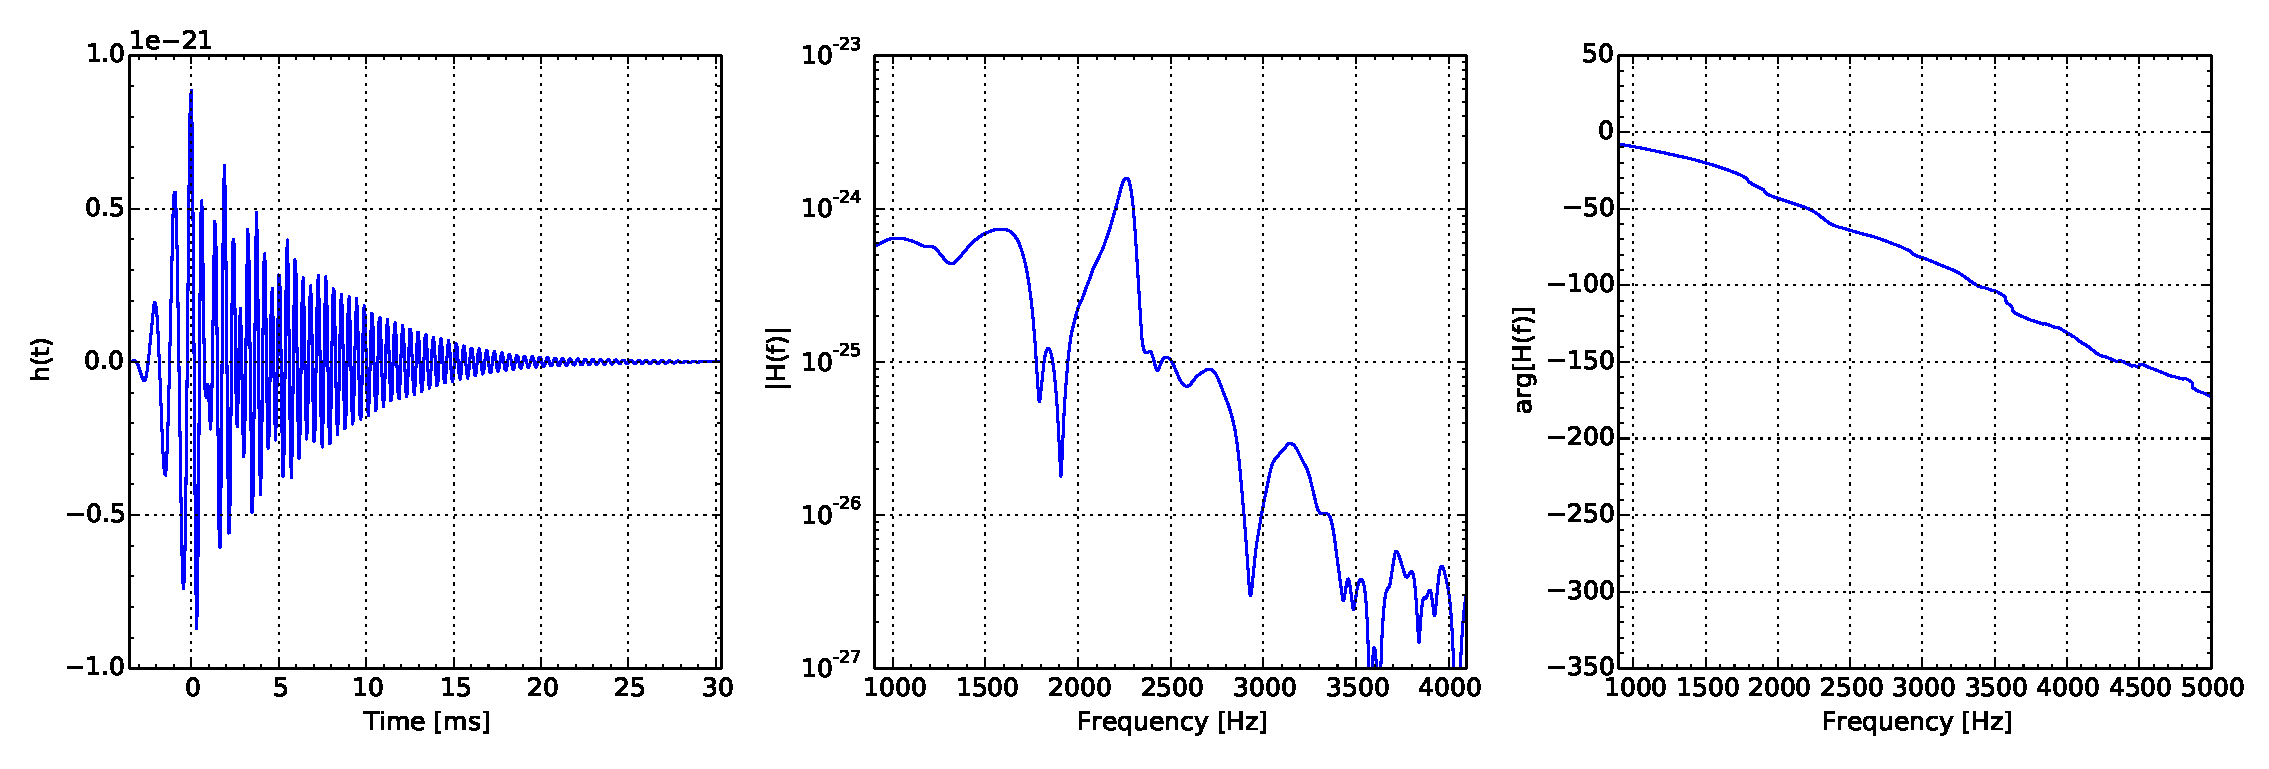
\includegraphics[width=\linewidth]{example_waveform.pdf}%
\end{minipage}


\subsection*{Previous and On-Going Analyses}


\section*{Principle Component Analysis \& Approximate Waveform Modelling}

\subsection*{Waveform Catalogue: Training Data}

\subsection*{Method: Feature Alignment \& PCA}

%
% Catalogue T-domain
%

%
% Catalogue F-domain
%
\begin{minipage}{\columnwidth}
\makeatletter
\newcommand{\@captype}{figure}
\makeatother
\centering
\subfloat[Catalogue Magnitudes]{%
  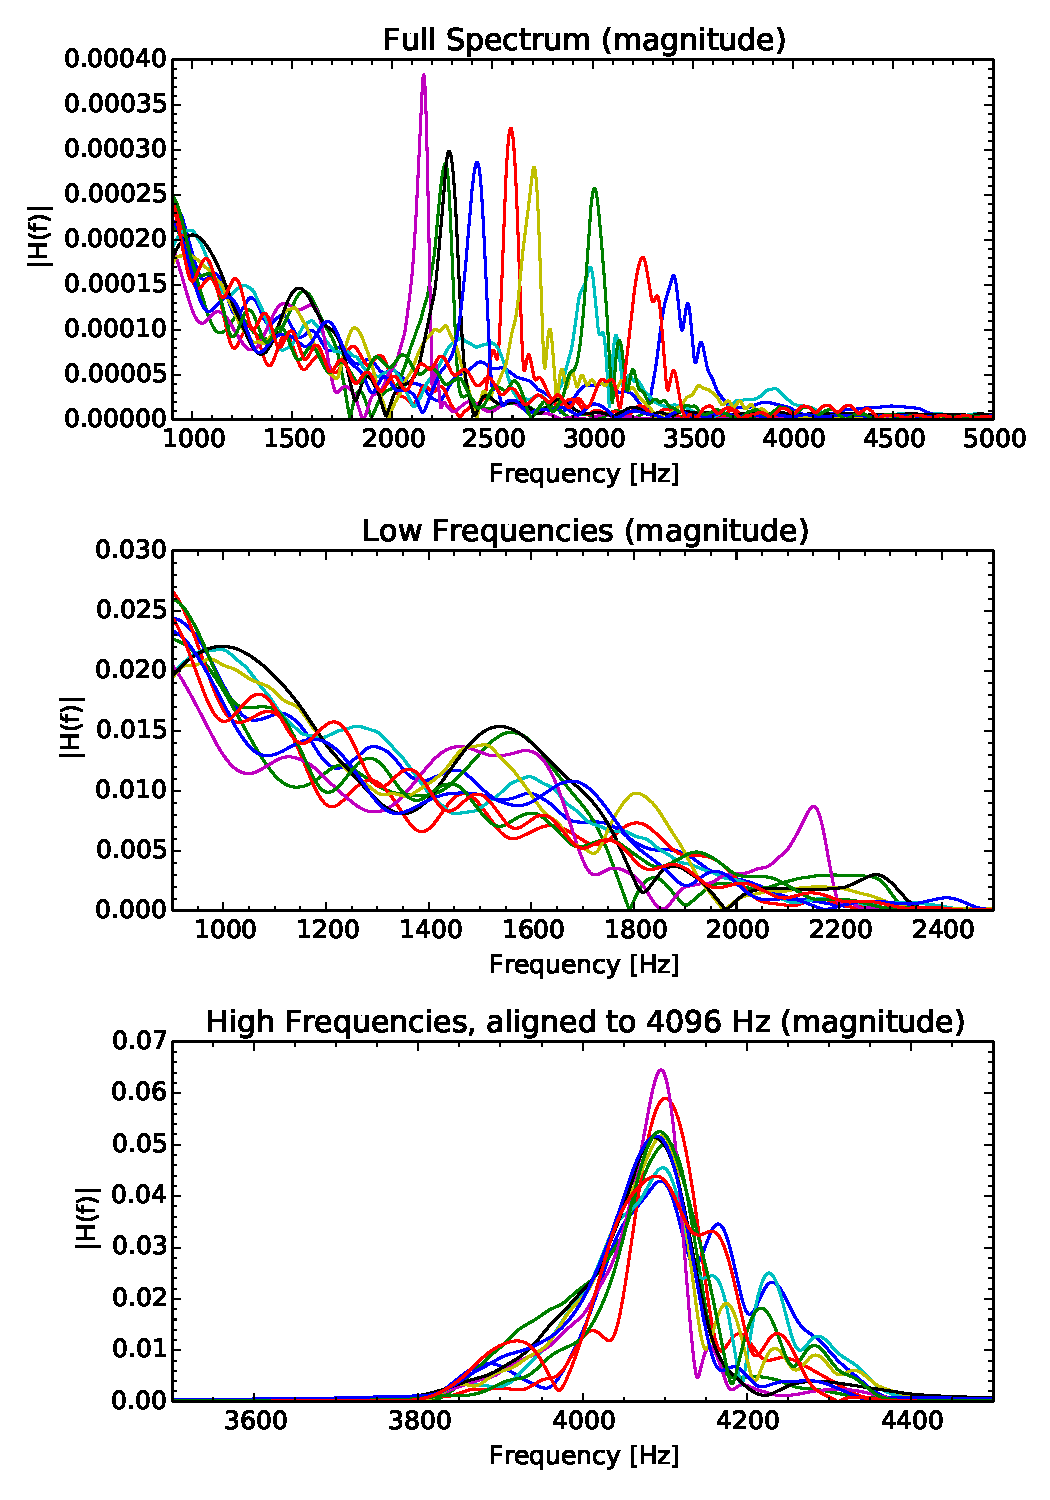
\includegraphics[width=0.4\linewidth]{catalogue_magnitude_overlay.pdf}%
  \label{fig:}%
}\qquad%
\subfloat[Catalogue Phases]{%
  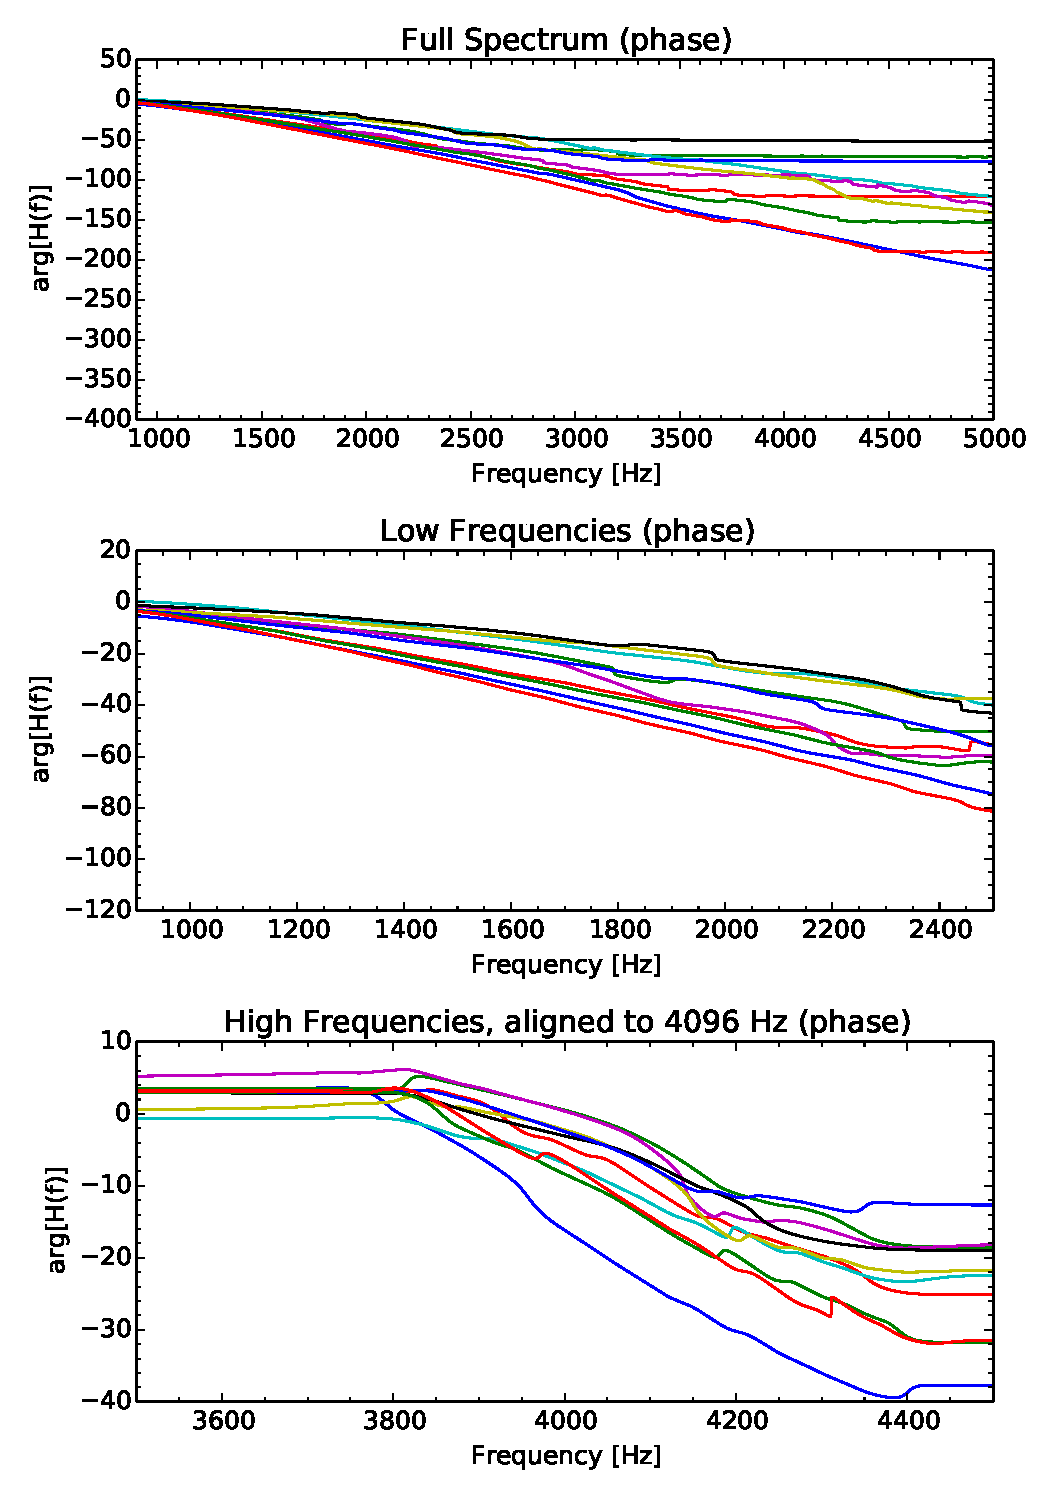
\includegraphics[width=0.4\linewidth]{catalogue_phase_overlay.pdf}%
  \label{fig:}%
}
\caption{Magnitude and phase spectra of our training data}
\end{minipage}

\subsection*{Results}

%
% PCs F-domain
%
\begin{minipage}{\columnwidth}
\makeatletter
\newcommand{\@captype}{figure}
\makeatother
\centering
\subfloat[PC Magnitudes]{%
  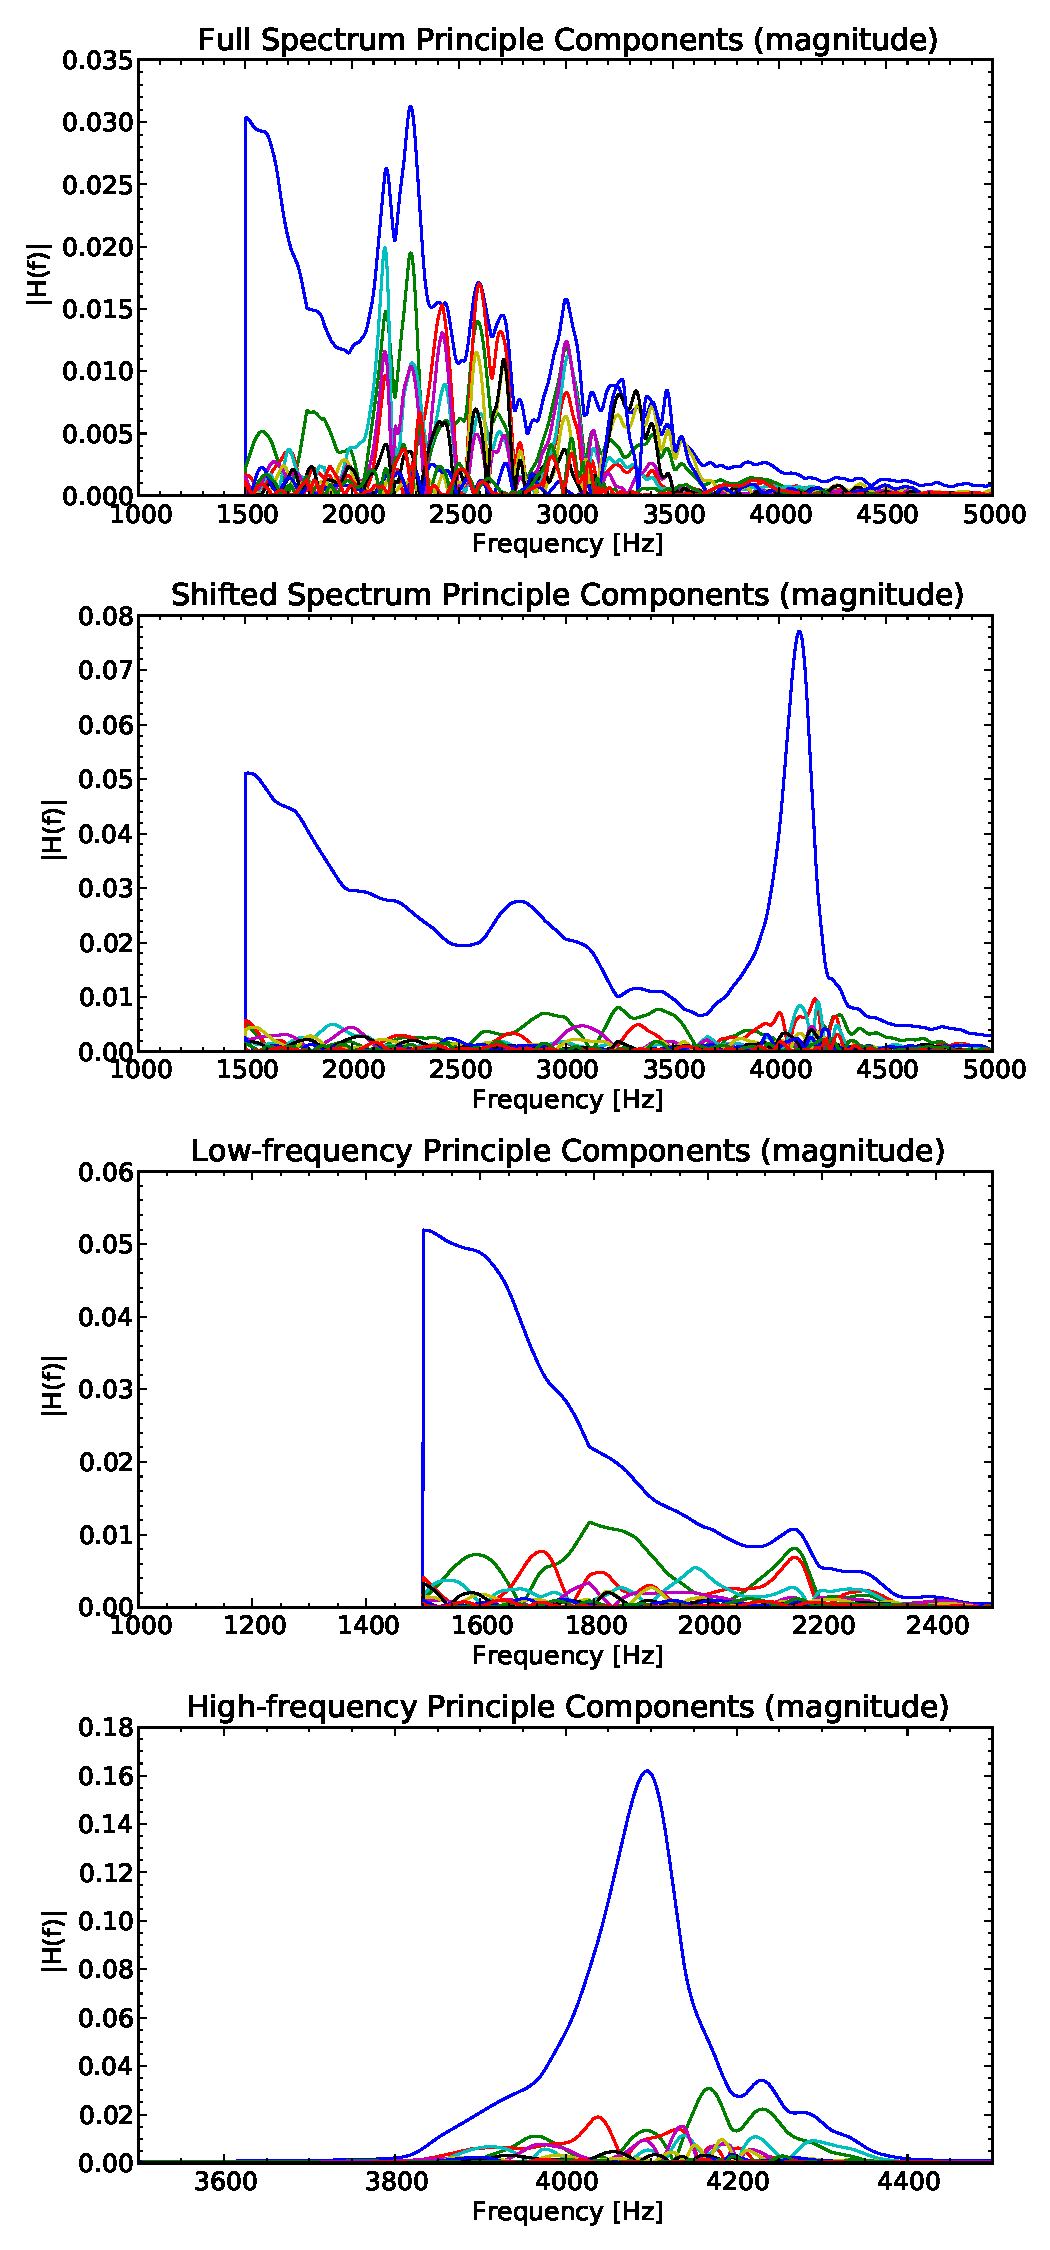
\includegraphics[width=0.4\linewidth]{pcs_magnitude_overlay.pdf}%
  \label{fig:}%
}\qquad%
\subfloat[PC Phases]{%
  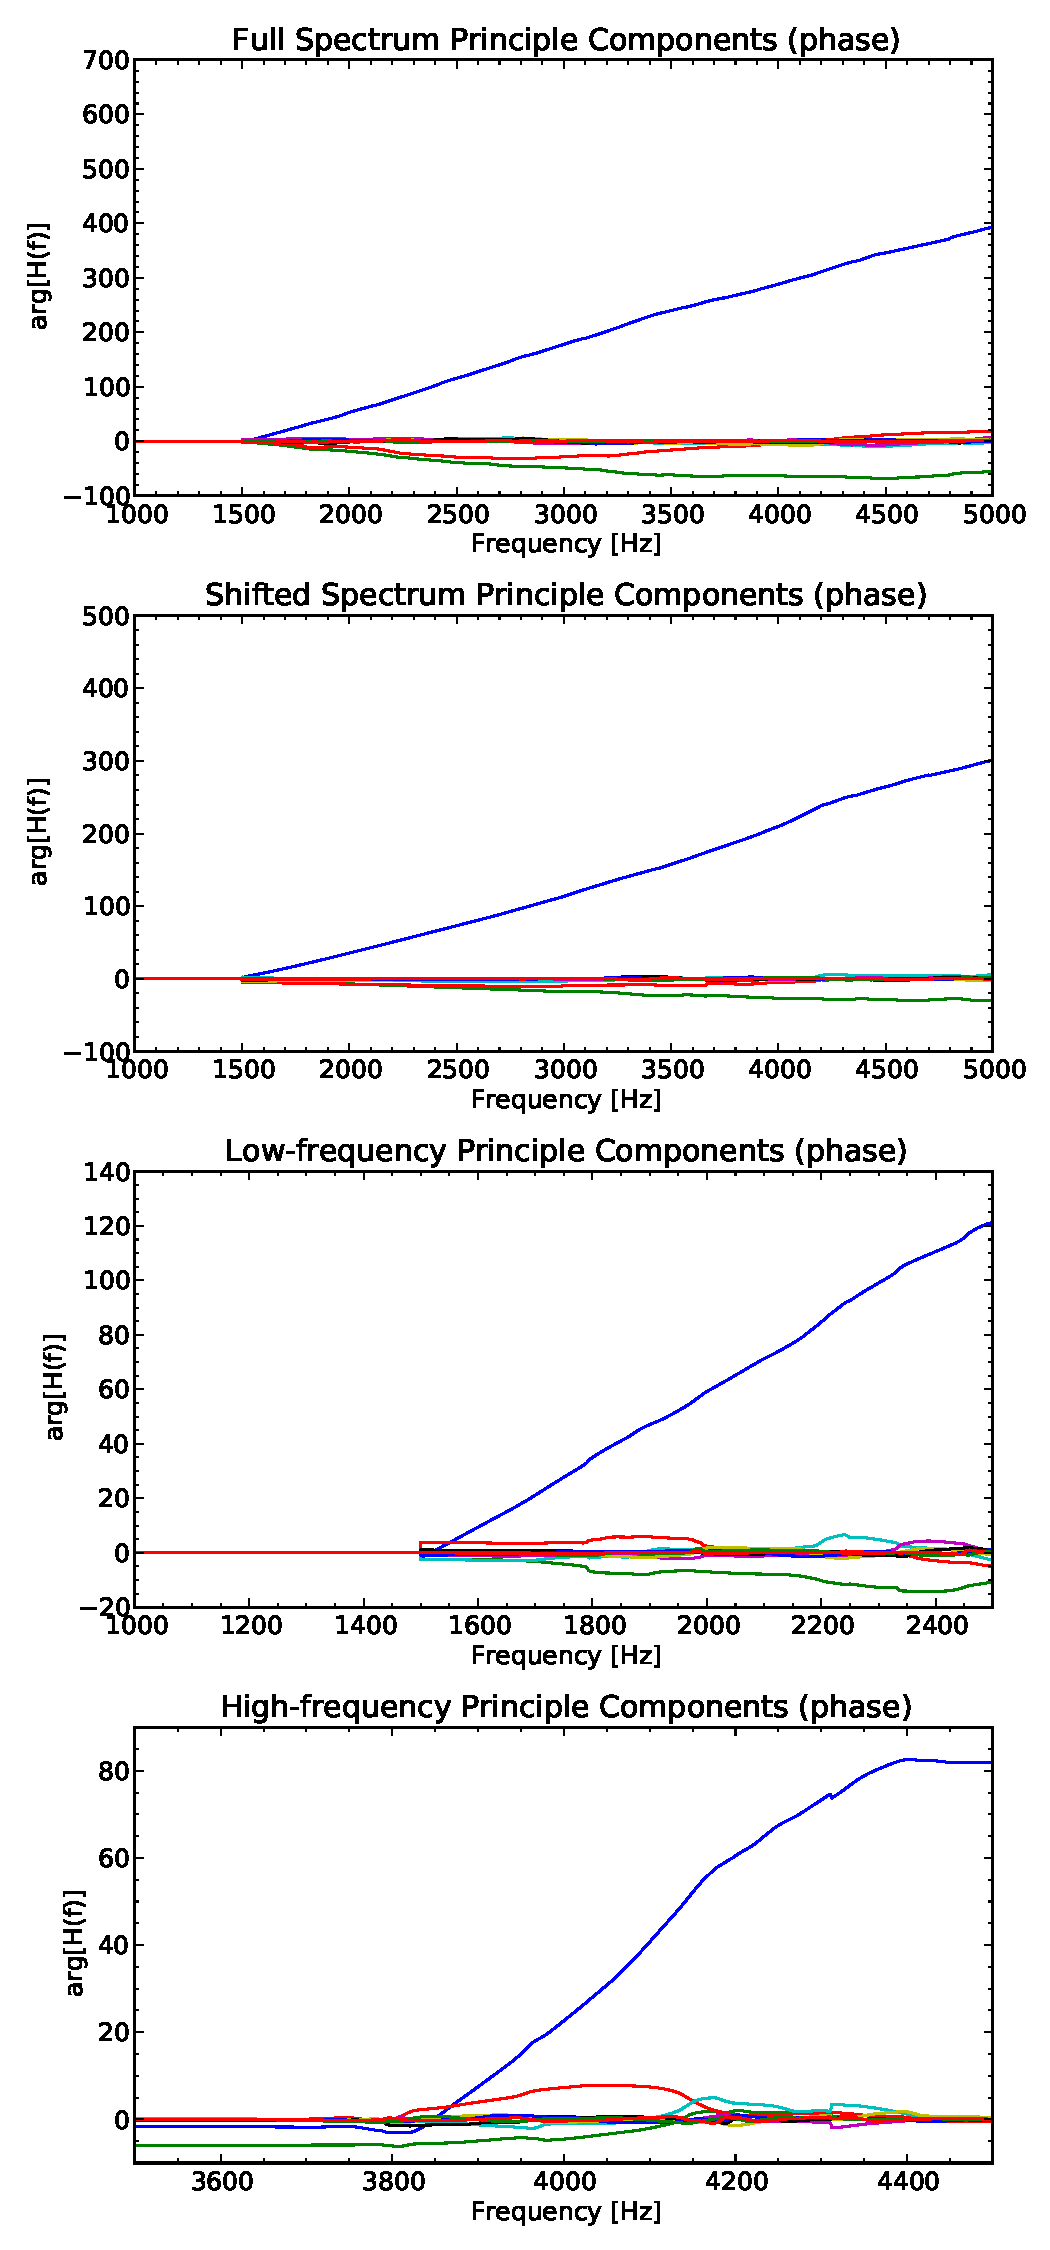
\includegraphics[width=0.4\linewidth]{pcs_phase_overlay.pdf}%
  \label{fig:}%
}
\caption{Magnitude and phase spectra of our principle component basis}
\end{minipage}


%
% Eigenergy and Ideal matches
%
\begin{minipage}{\columnwidth}
\makeatletter
\newcommand{\@captype}{figure}
\makeatother
\centering
\subfloat[Idealised match for full-spectrum PCs]{%
    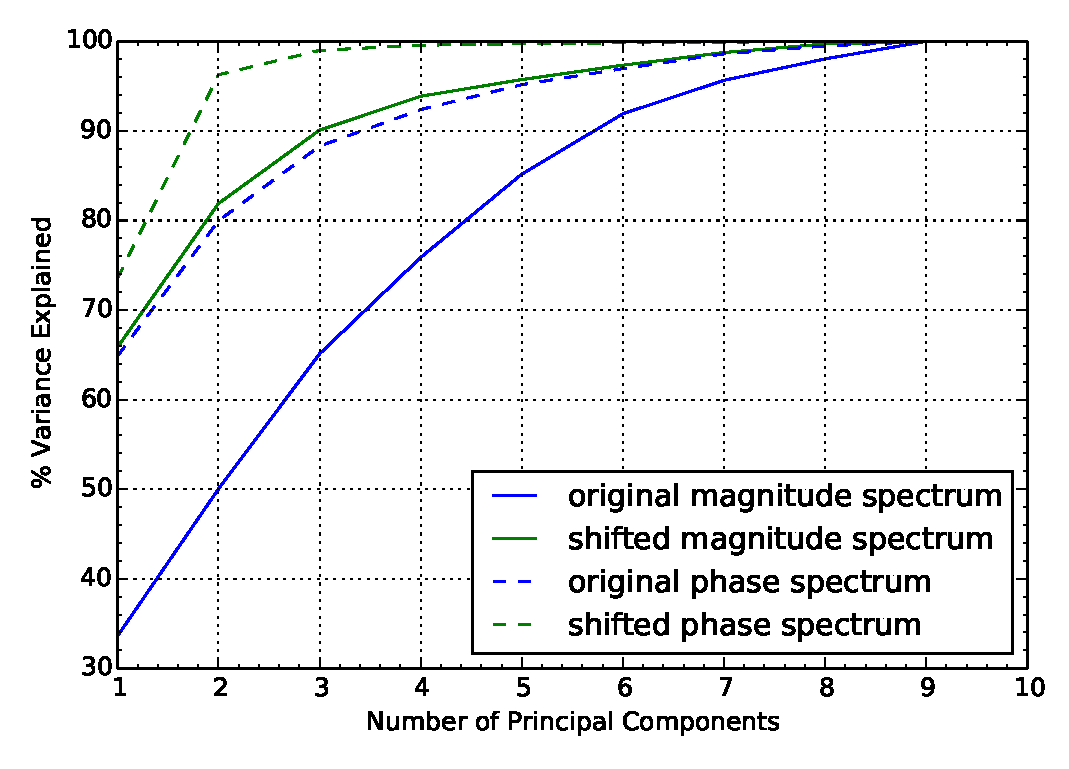
\includegraphics[width=0.4\linewidth]{eigenergy.pdf}%
  \label{fig:}%
}\qquad%
\subfloat[Idealised match for full-spectrum PCs]{%
  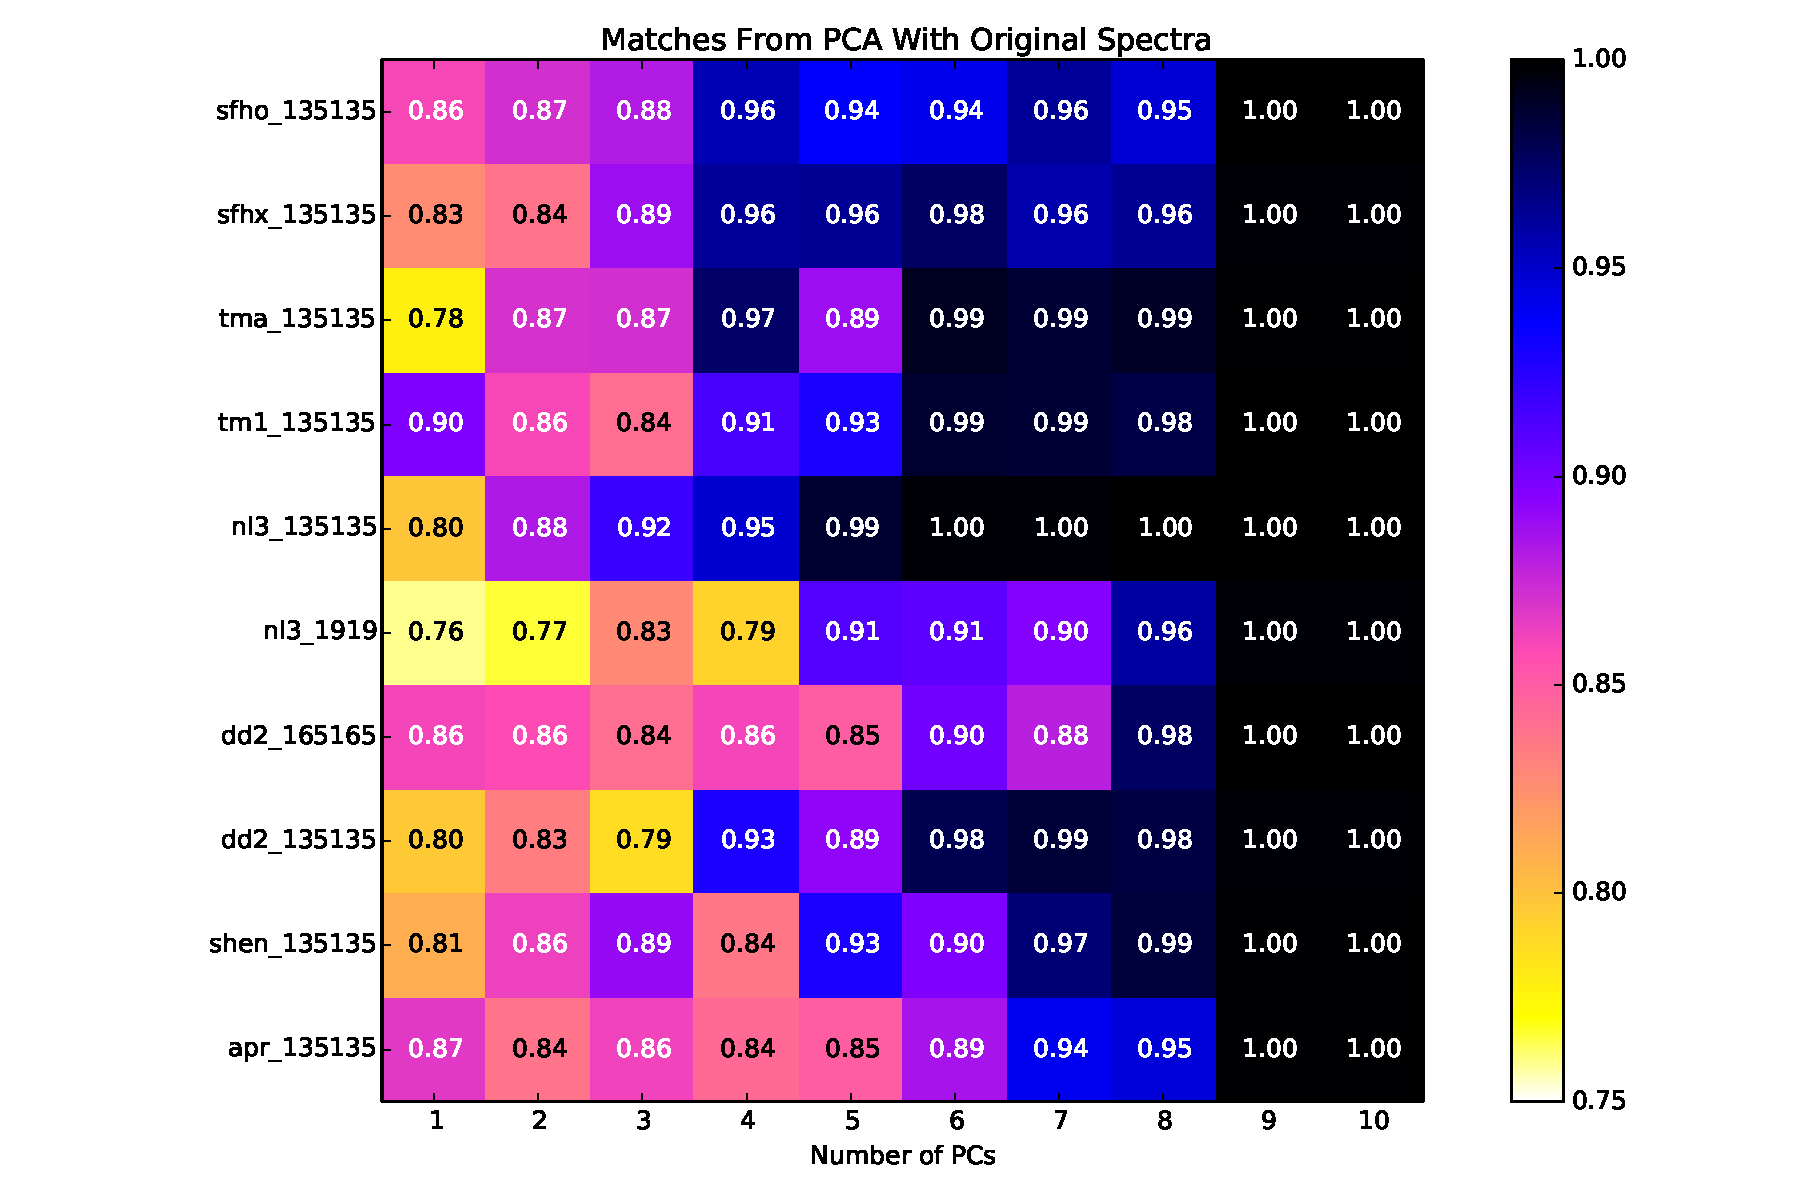
\includegraphics[width=0.45\linewidth]{fullspec_ideal_matches.pdf}%
  \label{fig:}%
}
\caption{\emph{Left}: matches for waveforms reconstructed using PCs based on
the full, unadulterated frequency content of the catalogue (no feature
alignment); \emph{Right}: matches for waveforms reconstructed using PCs based on
the full, \emph{shifted} frequency content of the catalogue}
\end{minipage}


\begin{minipage}{\columnwidth}
\makeatletter
\newcommand{\@captype}{figure}
\makeatother
\centering
\subfloat[Idealised match for `stiched' PCs]{%
  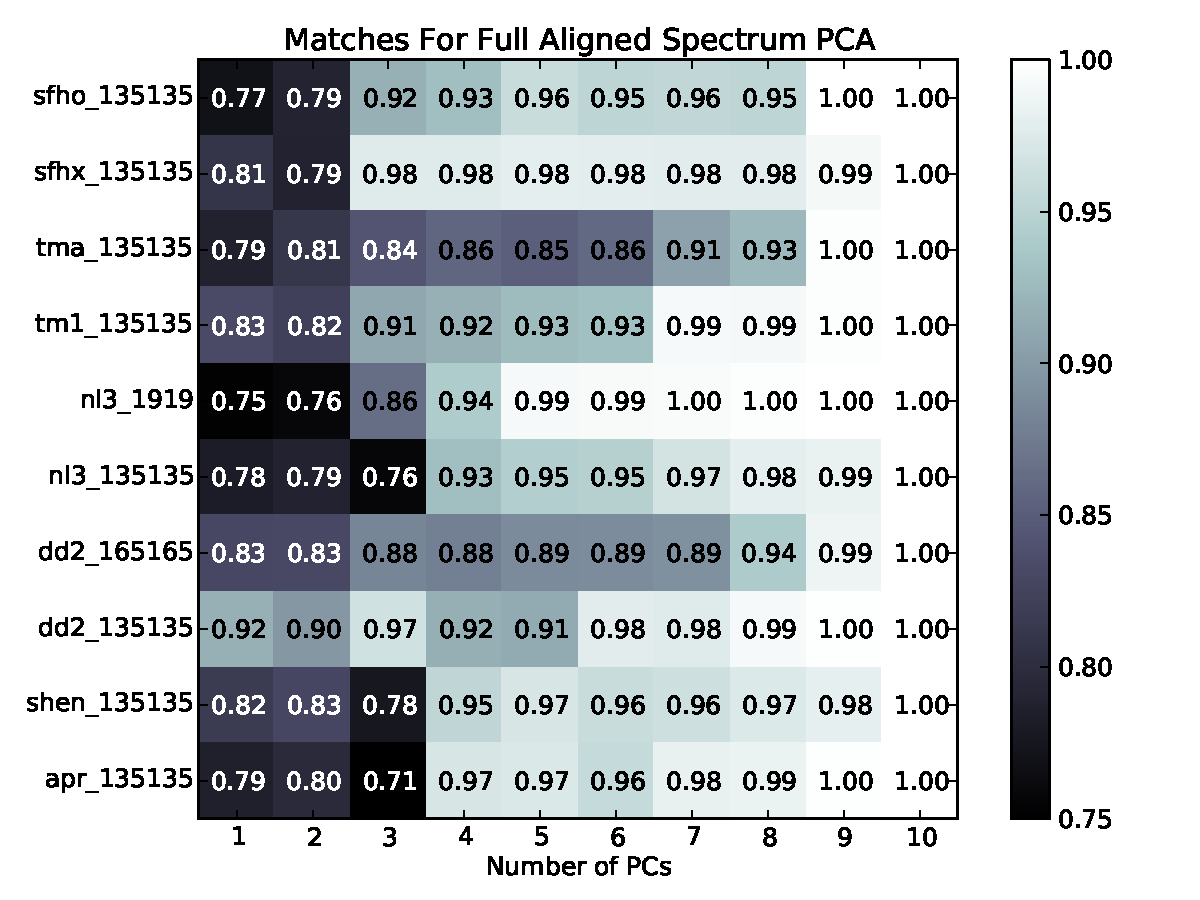
\includegraphics[width=0.45\linewidth]{shiftspec_ideal_matches.pdf}%
  \label{fig:}%
}\qquad%
\subfloat[Idealised match for `shifted' PCs]{%
  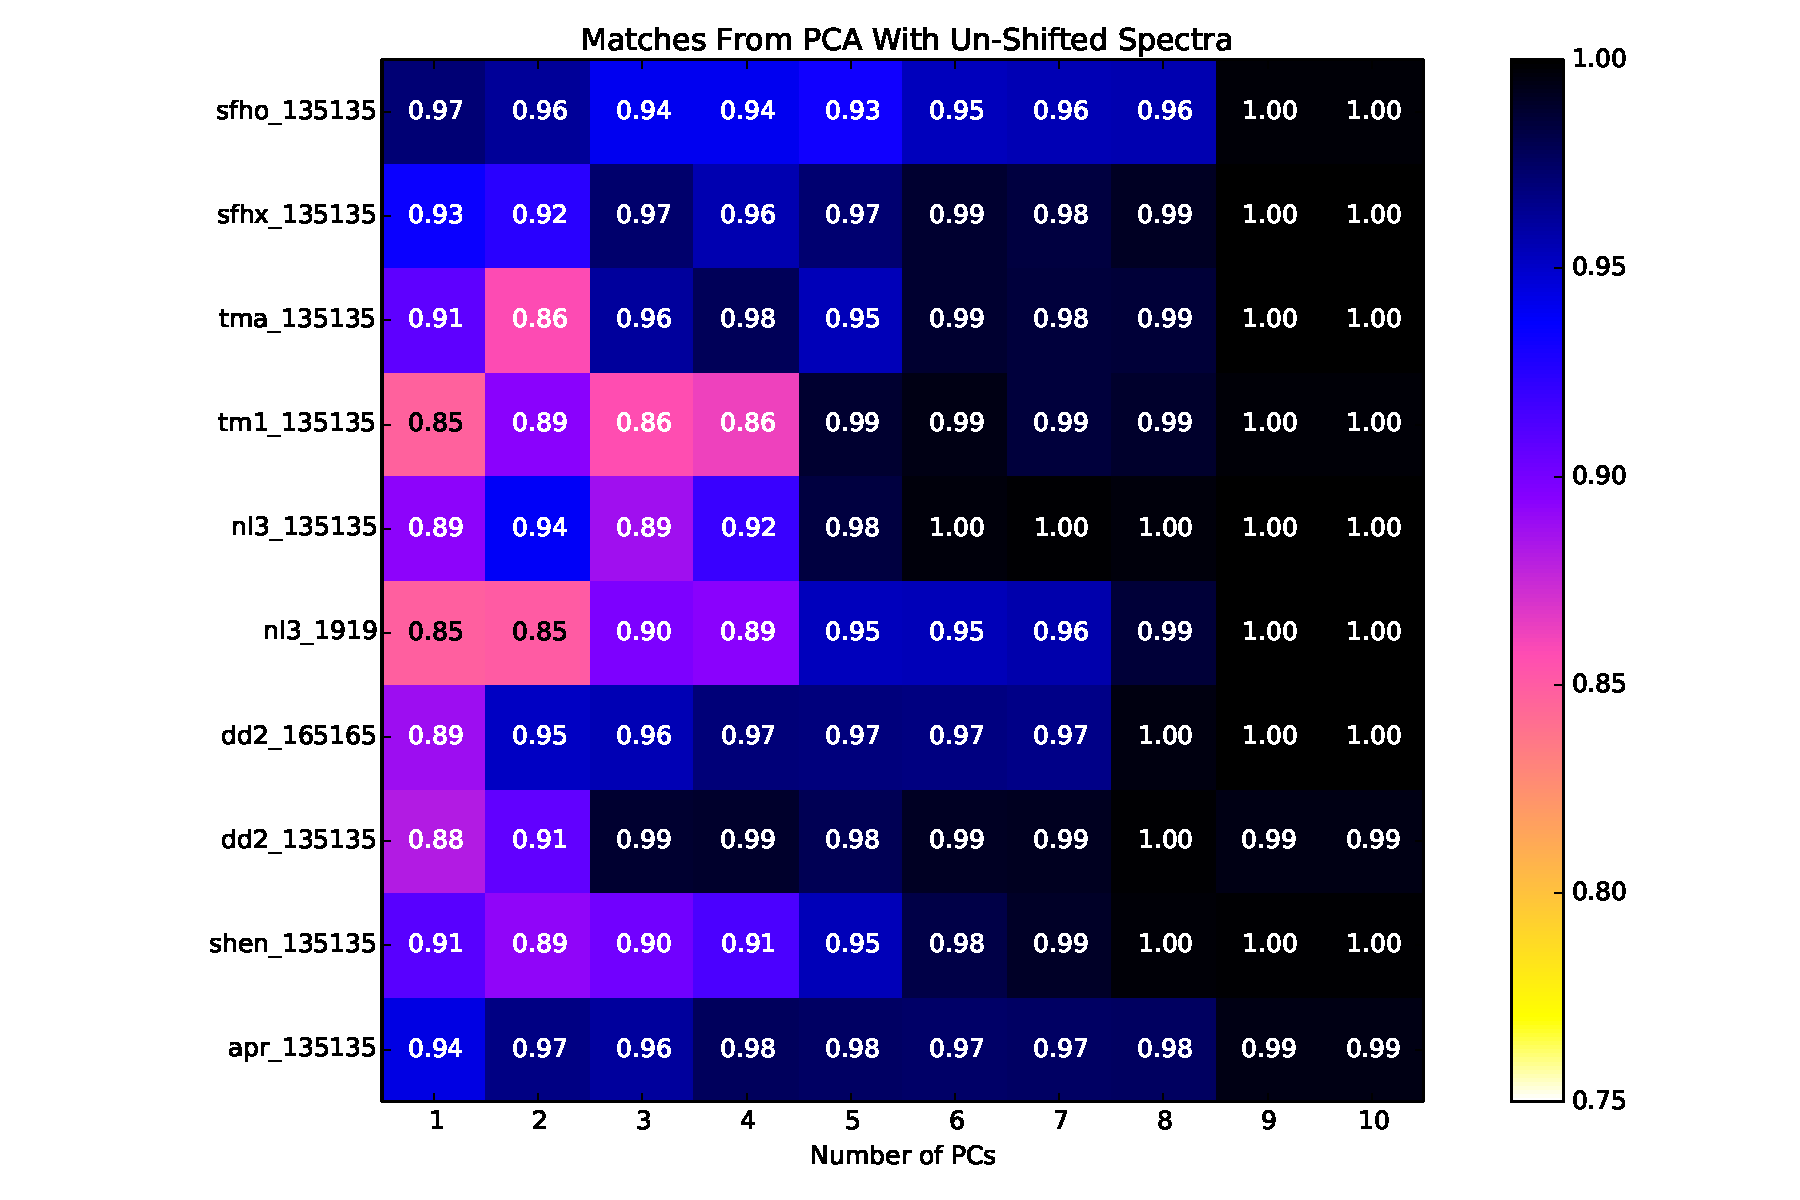
\includegraphics[width=0.45\linewidth]{unshiftspec_ideal_matches.pdf}%
  \label{fig:}%
}
\caption{Separate high and low frequency matches}
\end{minipage}

\begin{minipage}{\columnwidth}
\makeatletter
\newcommand{\@captype}{figure}
\makeatother
\centering
\subfloat[Idealised match for `stiched' PCs]{%
  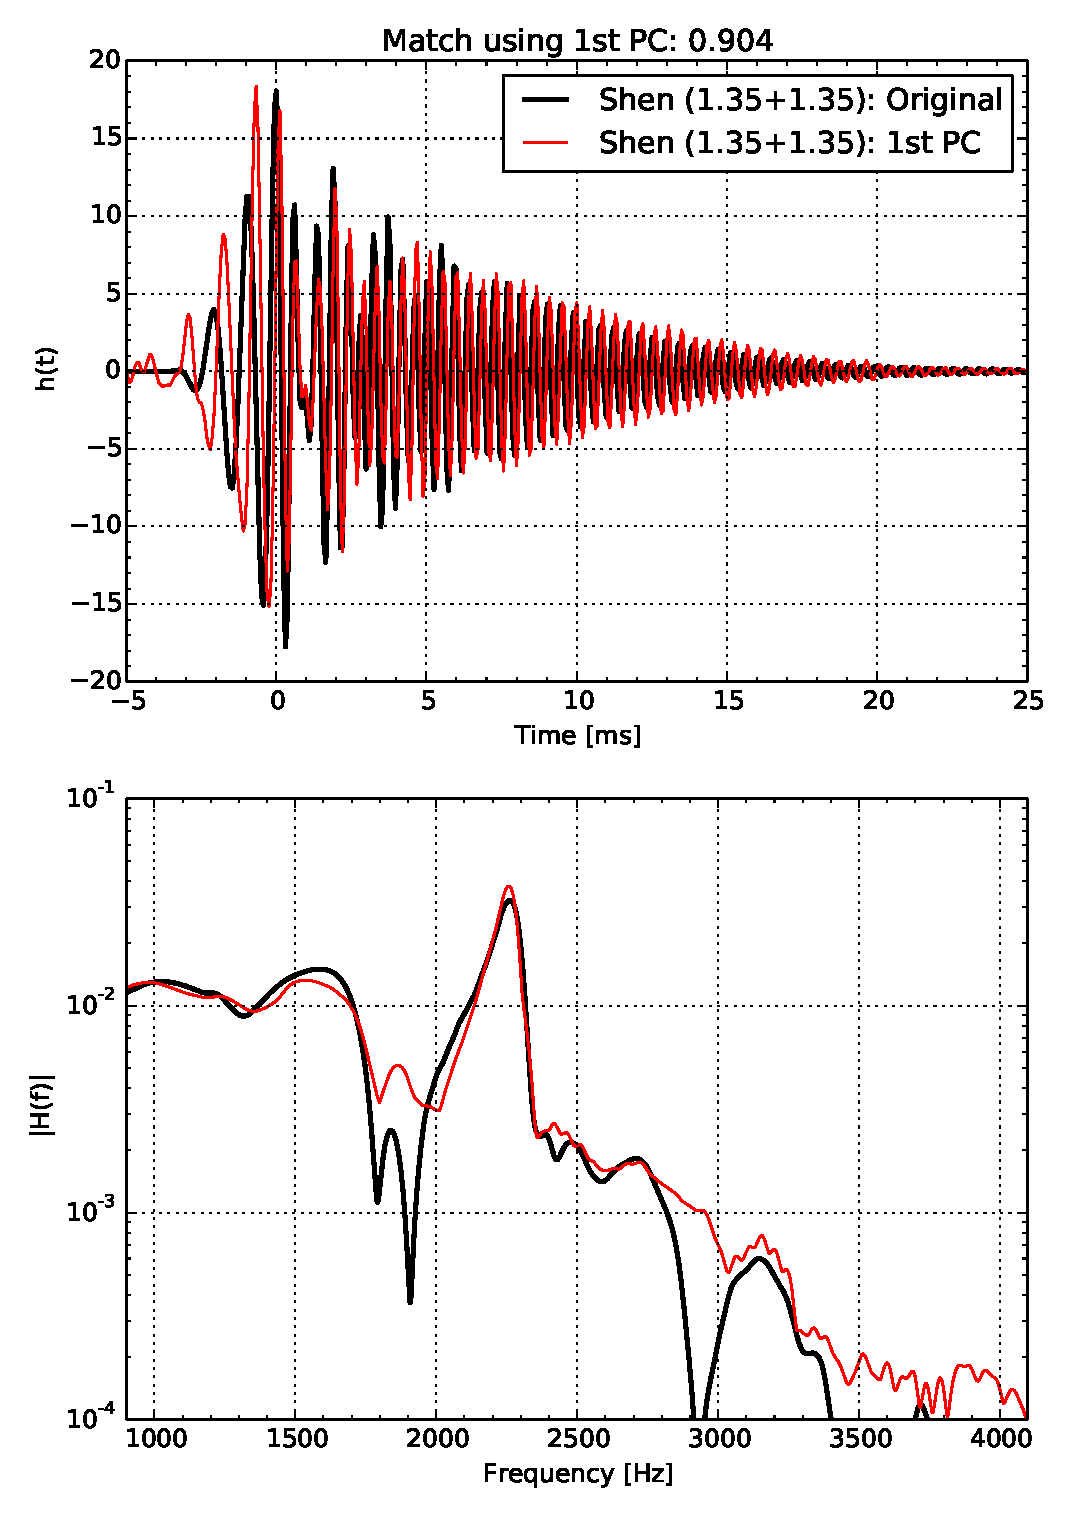
\includegraphics[width=0.4\linewidth]{firstPC_example_waveform_reconstruction.pdf}%
  \label{fig:}%
}\qquad%
\subfloat[Idealised match for `shifted' PCs]{%
  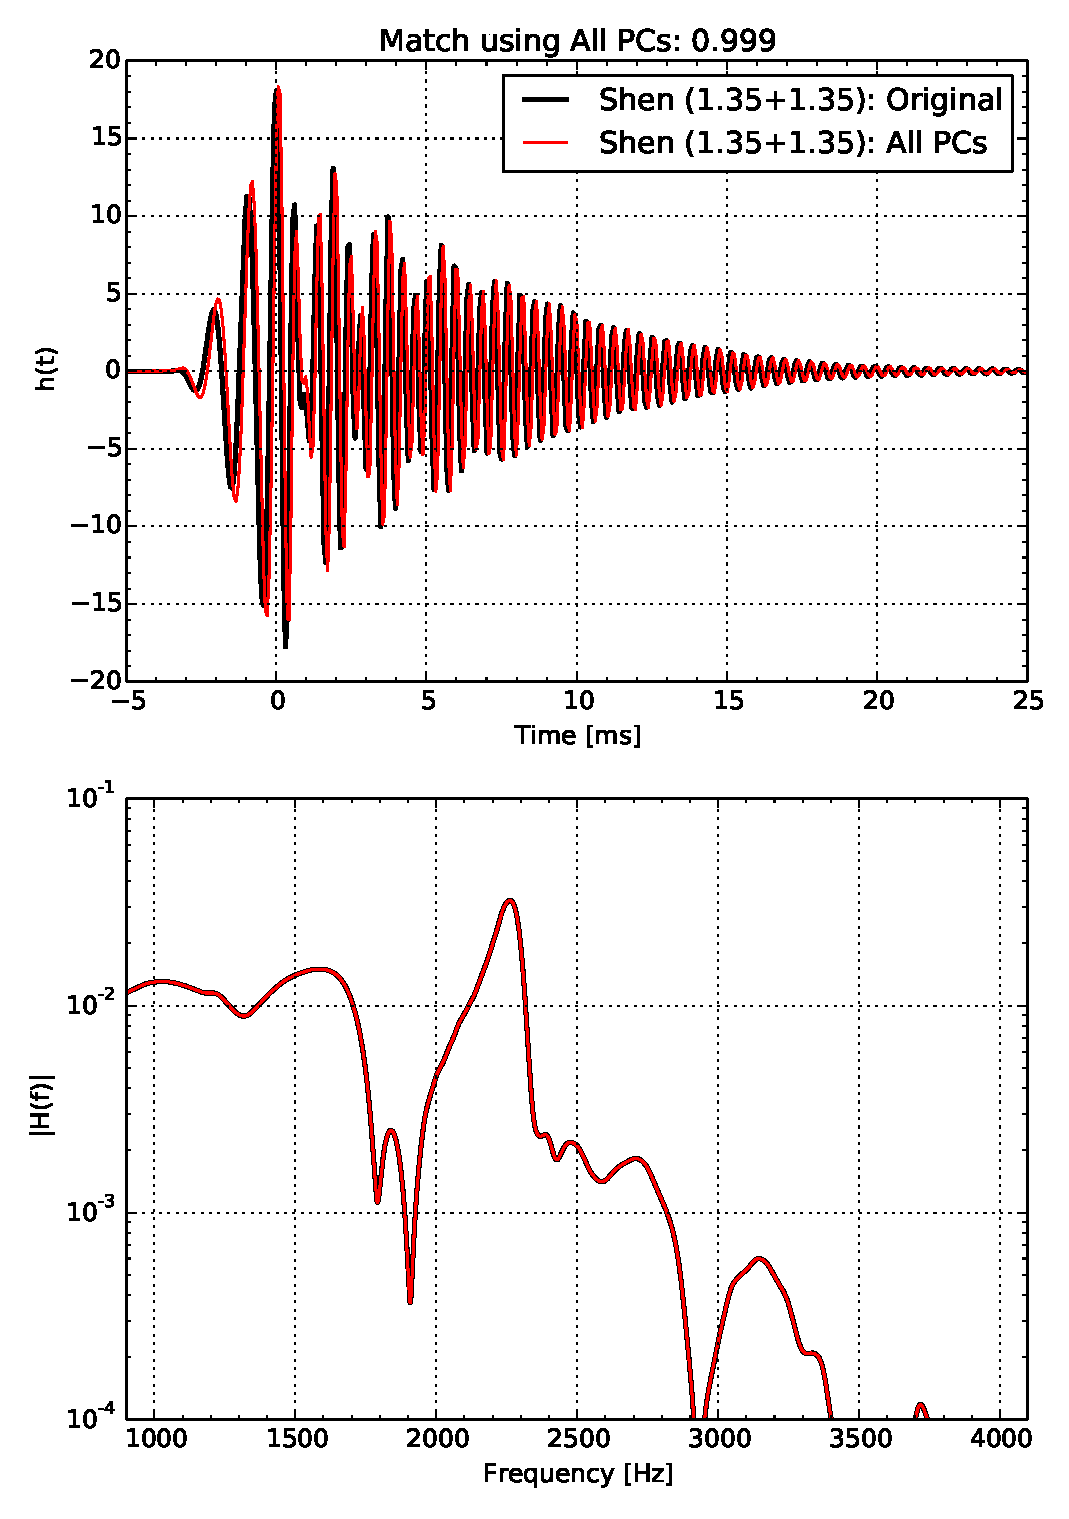
\includegraphics[width=0.4\linewidth]{allPCs_example_waveform_reconstruction.pdf}%
  \label{fig:}%
}
\caption{Separate high and low frequency matches}
\end{minipage}

%----------------------------------------------------------------------------------------
%	CONCLUSIONS
%----------------------------------------------------------------------------------------

\color{SaddleBrown} % SaddleBrown color for the conclusions to make them stand out

\section*{Applications \& Future Directions}

\begin{itemize}
\item Pellentesque eget orci eros. Fusce ultricies, tellus et pellentesque fringilla, ante massa luctus libero, quis tristique purus urna nec nibh. Phasellus fermentum rutrum elementum. Nam quis justo lectus.
\item Vestibulum sem ante, hendrerit a gravida ac, blandit quis magna.
\item Donec sem metus, facilisis at condimentum eget, vehicula ut massa. Morbi consequat, diam sed convallis tincidunt, arcu nunc.
\item Nunc at convallis urna. isus ante. Pellentesque condimentum dui. Etiam sagittis purus non tellus tempor volutpat. Donec et dui non massa tristique adipiscing.
\end{itemize}

\color{DarkSlateGray} % Set the color back to DarkSlateGray for the rest of the content


 %----------------------------------------------------------------------------------------
%	REFERENCES
%----------------------------------------------------------------------------------------

\nocite{*} % Print all references regardless of whether they were cited in the poster or not
\bibliographystyle{plain} % Plain referencing style
\bibliography{sample} % Use the example bibliography file sample.bib

%----------------------------------------------------------------------------------------
%	ACKNOWLEDGEMENTS
%----------------------------------------------------------------------------------------

\section*{Acknowledgements}

Etiam fermentum, arcu ut gravida fringilla, dolor arcu laoreet justo, ut imperdiet urna arcu a arcu. Donec nec ante a dui tempus consectetur. Cras nisi turpis, dapibus sit amet mattis sed, laoreet.

%----------------------------------------------------------------------------------------

\end{multicols}
\end{document}
